\documentclass[12pt,english]{article}

\setlength\parindent{0pt}
\usepackage{amssymb,amsmath,amscd,graphicx,fontenc,bbold,bm,amsthm,mathrsfs,mathtools}

\usepackage{algorithm, algorithmic}

% code and psendocode
\usepackage{verbatim}
\usepackage{minted}
\usemintedstyle{trac}

% colors
\usepackage{xcolor}
\definecolor{LightGray}{gray}{0.95}
\definecolor{DarkGray}{gray}{0}

\usepackage{minted} % code listing
\usemintedstyle{trac}

\definecolor{LightGray}{gray}{0.95}

% new commands
\newcommand{\code}[1]{{\small\colorbox{LightGray}{\texttt{#1}}}}
\newcommand{\tr}{\mathrm{Trace}}
\newcommand{\real}{\mathbb{R}}
\newcommand{\sigmoid}{\mathrm{sigmoid}}
\newcommand{\softmax}{\mathrm{softmax}}
\newcommand{\sign}{\mathrm{sign}}
\newcommand{\abs}{\mathrm{abs}}
\newcommand{\rect}{\mathrm{rect}}
\newcommand{\onehot}{\mathrm{onehot}}
\newcommand{\relu}{\mathrm{relu}}
\newcommand{\pd}[1]{\frac{\partial}{\partial {#1}}}

\usepackage[top=3cm,bottom=3cm,right=2.3cm,left=2.3cm,twoside=false]{geometry}

\title{Noisy image classification with CNN}
\author{Jonathan Guymont, Marzieh Mehdizadeh}

\date{}

\begin{document}

\maketitle

\section{Introduction}
The dataset contains $10,000$ images of $31$ different categories in both the training and the testing set. Random noise had been added to the images, making the task more challenging. Our goal was to classify the images using an appropriate algorithm. We also tried to de-noise the images before feeding them to the model. Our baseline algorithm was the multinomial logistic regression, formally:
\begin{equation}
p(y=j|\bm{x})
= \frac{e^{\bm{x}^{T}\mathbf{W}_{\cdot, j}+\mathbf{b}}}{\sum_{k} e^{\bm{x}^{T}\mathbf{W}_{\cdot, k}+\mathbf{b}}} 
\quad 
j= 1,\cdots ,31.
\label{softmax}
\end{equation}
The second approach we used is the most popular architecture used for image classification which is Convolutional Neural Networks (CNNs).

\section{Feature Design}
\textbf{Preprocessing.} First we have the preprocessing step to have a better quality input images to feed to our models. We used the Gaussian-filter to denoise the images, the Gaussian smoothing operator is a 2-D convolution operator that is used to blur images and remove detail and noise. In this sense it is similar to the mean filter, but it uses a different kernel that represents the shape of a Gaussian (bell-shaped) hump, (we use cropping and resizing, but it did not have a good influence on out result). We used the preprocessed data to feed to our models, each de-noised image's pixel  is a feature so we have $100\times 100= 10^4$ feature to feed each model described as below.\\

\textbf{Data augmentation.} We also augmented the size of the dataset by \textit{flipping} 40\% of the images and adding them to the training set.\\

\textbf{Convolution layers.} Since the convolutional layers present in the CNN can be seen as feature extractor, we discuss there effect in this section. Filters (or kernels) consist of (randomly initialized) trainable parameters depending on the depth and filters at each layer of a network. The filters convolve on each image's pixel to create some feature/activation maps at each layer. During this process, (through back-propagation) they learn by adjusting those initial values to capture the correct magnitude of a spatial feature on which they are convolving. These high number of filters essentially learn to capture features from images based on the learned magnitude. Hence they can successfully boil down a given image into a highly abstracted representation which is easy for predicting.

\section{Algorithm}
We used a logistic regression as our baseline model. The probabilities of each class given an input $\bm{x}$ are obtained using equation \ref{softmax}, where $\mathbf{W}$ and $\mathbf{b}$ are trained parameters. When making prediction, the class with the highest output probability is predicted. We added L2 regularization to the loss function to prevent the model from overfitting. Still the performance of this model was very low. This model does not have hyperparameter. We trained the model using stochastic gradient descent with the negative log-likelihood loss. The training parameters for the logistic regression are shown in table \ref{table:lr_hyper}.\\
\begin{table}[h!]
	\centering
	\begin{tabular}{|c|c|c|c|c|}
		\hline 
		learning rate & momentum & weight decay & epochs & batch size \\ 
		\hline 
		0.001 & 0 & 0.001 & 1000 & 64\\ 
		\hline 
	\end{tabular} 
	\caption{Training hyperparameters of the logistic regression}
	\label{table:lr_hyper}
\end{table}

The second classifier we used is a CNN with a softmax linear layer at the end to output the probabilities. In other words, we used convolutions layers to improve the features before feeding them to a multinomial logistic regression classifier.  The model architecture was composed of 4 convolution layers, followed by a linear hidden layer, and the softmax linear output layer. The outputs of the convolutions were flatten and concatenate together to form a unique vector before feeding them to the linear layer. Each convolution layer was followed immediately by a relu activation function. We normalized the batch and applied dropout at each convolution layer. The dropout rate was set to 0.5 when the images were not denoised and 0.3 when the image where denoised - we used different dropout because we assume denoised image needed less regularization since the model was less likely to fit random noise. Each convolution layer outputs 32 matrix. We used strike of 3 and max pooling of 2 to slowly reduce the dimension of the features hoping that by compressing the features, some noise would be removed. The philosophy behind this choice of architecture was to have enough capacity to learn to discriminate complex images while also having enough regularization to prevent the model from learning the noise. The performance of this model was better then the baseline - this was expected since it had larger capacity and it was easier to regularize with the use of dropout and batch normalization. We also used SGD with negative log-likelihood loss to train this model. The training hyperparameters of this model are shown in table \ref{table:cnn_hyper}.

\begin{table}[h!]
	\centering
	\begin{tabular}{|c|c|c|c|c|}
		\hline 
		learning rate & momentum & weight decay & epochs & batch size \\ 
		\hline 
		0.001 & 0.9 & 0 & 1000 & 64\\
		\hline 
	\end{tabular} 
	\caption{Training hyperparameters of the CNN}
	\label{table:cnn_hyper}
\end{table}

\section{Methodology}
We used a train/valid split of 0.8/0.2. For the CNN, we tested 9 different models-data configuration: three different set of hyperparameters each tested with 3 different preprocessing. The selected architecture is described in figure \ref{fig:cnn}. The difference between the datasets was the preprocessing applied and whether there was data augmentation (see the features section for more details). The model that perform best on the validation set was chosen. For the logistic regression, we tested we 3 different weight decay: 0.1, 0.01, 0.001.

\section{Results}
Accuracies for both models are shown in table \ref{table:acc}. Both models were train for one thousand epochs. The CNN classifier was generalizing a lot more then the logistic regression. Figure \ref{fig:acc} and \ref{fig:loss} show the accuracy of the selected CNN over both the training set and the validation set. Augmenting the data helped us gain 2\% on the validation set (from $\sim 60$ to $\sim 62$) but de-noising the data didn't improve the accuracy, though the model was training faster on the de-noised data. It is possible that a using learning rate schedule instead of a constant learning rate would have prevent the model from plateauing as fast. 


\begin{table}[h!]
	\centering
	\begin{tabular}{|c|c|c|}
		\hline 
		model & training & validation\\ 
		\hline 
		CNN & 73.33 & 62.79 \\ 
		\hline 
		logistic regression & 97.27 & 8.46\\
		\hline
	\end{tabular} 
	\caption{Validation and train accuracy of the selected CNN classifier (describe in figure \ref{fig:cnn}) and the baseline logistic classifier after 1000 iteration of training.}
	\label{table:acc}
\end{table}

\begin{figure}
\begin{minted}[bgcolor=LightGray, fontsize=\footnotesize]{python}
Classifier(
  (conv): Sequential(
    (batch_norm0): BatchNorm2d(1, eps=1e-05, momentum=0.1, affine=True, track_running_stats=True)
    (conv1): Conv2d(1, 32, kernel_size=(3, 3), stride=(1, 1), padding=1)
    (relu1): ReLU()
    (max_pool1): MaxPool2d(kernel_size=2, stride=2, padding=0, dilation=1, ceil_mode=False)
    (dropout1): Dropout(p=0.3)
    (batch_norm1): BatchNorm2d(32, eps=1e-05, momentum=0.1, affine=True, track_running_stats=True)
    (conv2): Conv2d(32, 32, kernel_size=(3, 3), stride=(1, 1), padding=1)
    (relu2): ReLU()
    (max_pool2): MaxPool2d(kernel_size=2, stride=2, padding=0, dilation=1, ceil_mode=False)
    (dropout2): Dropout(p=0.3)
    (batch_norm2): BatchNorm2d(32, eps=1e-05, momentum=0.1, affine=True, track_running_stats=True)
    (conv3): Conv2d(32, 32, kernel_size=(3, 3), stride=(1, 1), padding=1)
    (relu3): ReLU()
    (max_pool3): MaxPool2d(kernel_size=2, stride=2, padding=0, dilation=1, ceil_mode=False)
    (dropout3): Dropout(p=0.3)
    (batch_norm3): BatchNorm2d(32, eps=1e-05, momentum=0.1, affine=True, track_running_stats=True)
    (conv4): Conv2d(32, 32, kernel_size=(3, 3), stride=(1, 1), padding=1)
    (relu4): ReLU()
    (max_pool4): MaxPool2d(kernel_size=2, stride=2, padding=0, dilation=1, ceil_mode=False)
    (dropout4): Dropout(p=0.3)
    (batch_norm4): BatchNorm2d(32, eps=1e-05, momentum=0.1, affine=True, track_running_stats=True)
  )
  (dense): Sequential(
    (fc1): Linear(in_features=512, out_features=64, bias=True)
    (relu1): ReLU()
    (dropout1): Dropout(p=0.5)
    (fc2): Linear(in_features=64, out_features=31, bias=True)
    (softmax): LogSoftmax()
  )
  (loss_function): NLLLoss()
)
\end{minted}
	\caption{CNN classifier architecture (in Pytorch API)}
	\label{fig:cnn}
\end{figure}

\begin{figure}
	\centering
	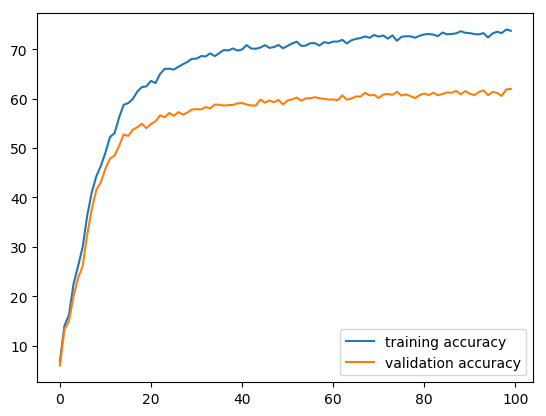
\includegraphics[scale=0.5]{../figures/accuracy_cnn_02.png}
	\caption{Accuracy of the classifier throughout epochs. One unit on the horizontal axis is equivalent to 10 epochs.}
	\label{fig:acc}
\end{figure}

\begin{figure}
	\centering
	\includegraphics[scale=0.5]{../figures/loss_cnn_02.png}
	\caption{Loss throughout the training of the CNN classifier. One unit on the horizontal axis is equivalent to 10 epochs.}
	\label{fig:loss}
\end{figure}

\section{Discussion}
The performance of the CNN model was much better that the performance of the multinomial logistic regression model.This result was expected since the CNN model have more capacity then the logistic regression and the CNN is more appropriate for image related task because of its filtering mechanism. We achieve a relatively good accuracy given how noisy the images were.  We didn't have access to significant computational power so we were not able to see if a very deep model would be able to distinguish the noise better by himself. The use of pretrained filters (trained for image related task) for the convolution layers would probably help since they would allow the model to recognize non-noisy shape from the beginning.

\end{document}